%% Documentclass:
%% Network Neuroscience
%\documentclass[finalfonts,NETN]{stjour}
\documentclass[NETN]{stjour}

%% or 

%% Manuscript, for double spaced, larger fonts
%\documentclass[manuscript]{stjour}
%% Only needed if you use `manuscript' option
% \journalname{Network Neuroscience}


%%%%%%%%%%% Article Set-Up %%%%%%%%%%%%%%%%%%%%%%%%%%%%%%%%%%%%
%% Article Type:
%% Default is Research.

%% Or, choose one of these options:
%% Research, Methods, Data, Review, and Perspective

\articletype{Research Article}

%%%%%%%%%%% Please supply information %%%%%%%%%%%%%%%%%%%%%%%%%

\supportinginfo{dx.doi.org/10.7910/DVN/PQ6ILM}

%% if no conflicts, this command doesn't need to be used
%% \conflictsofinterest{}

%%%%%%%%%%% to be supplied by MIT Press, only %%%%%%%%%%%%%%%%%
\citation{Betzel, R. F., Fukushima, M.,
He, Ye,
Zuo, Xi-Nian,
Sporns, O. (2016)\\
Dynamic fluctuations coincide with periods of high and low modularity
in resting-state functional brain  networks\\
Network Neuroscience, 1
}

\received{20 October 2016}
\accepted{7 November 2016}
\published{26 January 2016}
\setdoi{10.1162/NETN-00001} %% ???

\handlingeditor{Xi-Nian Zuo}

%%%%%%%% End MIT Press commands %%%%%%%%%%

%%%%%%%%%%%%%%%%%%%%%%%%%%%%%%%%%%%%%%%%%%%%%%%%%%%%%%%%%%%%%%%
%% author definitions should be placed here:

%% example definition
\def\taupav{\tau_{\mathrm{Pav}}}

\begin{document}
\title[Co-citations in context]{Co-citations in context}
\subtitle{disciplinary heterogeneity is relevant}

%% If shortened title for running head is needed so that the article title can fit
%%   in the running head, use [] argument, ie,
%%
%%   \title[Shortened Title for Running Head]{Title of Article}
%%   \subtitle{Subtitle Here}

%% Since we use \affil{} in the argument of the \author command, we
%% need to supply another version of the author names, without \affil{}
%% to be used for running heads:

\author[Author Names]
{James Bradley\affil{1},
Sitaram Devarakonda\affil{2}, Avon Davey\affil{2}, Dmitriy Korobskiy\affil{2}, Siyu Liu\affil{2}, Djamil Lakhdar-Hamina\affil{2},Tandy Warnow\affil{3}
\and George Chacko\affil{2}}

\affiliation{1}{Raymond A. Mason School of Business, College of William and Mary, Williamsburg, VA, USA}
\affiliation{2}{Netelabs, NET ESolutions Corporation, McLean, VA 22102, USA}
\affiliation{3}{Department of Computer Science, University of Illinois at Urbana-Champaign, Champaign, IL 61820, USA}


%ie.
%\affiliation{1}{Gatsby Computational Neuroscience Unit, University
%College London, London, United Kingdom} 

%\affiliation{2}{Another Department, Institution, City, Country}

%ie
%\affiliation{2}{Center for Studies in
%Behavioral Neurobiology, Concordia University, Montreal, Quebec,
%Canada}

\correspondingauthor{George Chacko}{netelabs@nete.com}

% ie,
%\correspondingauthor{Ritwik K. Niyogi}{ritwik.niyogi@gatsby.ucl.ac.uk}

\keywords{(co-citation analysis, bibliometrics, random graphs )}

%ie
%\keywords{work, leisure, normative, microscopic,  reinforcement learning, economics}

\begin{abstract}
Citation analysis of the scientific literature has been used to study and define disciplinary boundaries, to trace the dissemination of knowledge, and to estimate impact. Co-citation, the frequency with which pairs of publications are cited, provides insight into how documents relate to each other and across fields. Co-citation analysis has been used to characterize combinations of prior work as conventional or innovative and to derive features of highly cited publications. Given the organization of science into disciplines, a key question is the sensitivity of such analyses to frame of reference. Our study examines this question using  semantically-themed citation networks. We observe that trends reported to be true across the scientific literature do not hold for focused citation networks, and we conclude that co-citation analysis requires a contextual perspective.
\end{abstract}

% \begin{authorsummary} 
% \end{authorsummary}
\section{Introduction}

Citation and network analysis of  scientific literature reveals information on semantic relationships between publications, collaboration between scientists, and the practice of citation itself~\citep{garfield_citation_1955,de_solla_price_networks_1965,newman_structure_2001,Shi:2010:CHI:1816123.1816131,patience_pmid28560354}. Co-citation, the frequency with which two documents are cited together in other documents provides additional insights, including the identification of semantically related documents, fields, specializations, and new ideas in science~\citep{small_co-citation_1973, marshakova-shaikevich_co-citation_1973,boyack_co-citation_2010, 10.3389/frma.2018.00020}. 

\citep{uzzi_atypical_2013} used a novel approach for co-citation analysis using, as input, 17.9 million articles and their cited references, from the Web of Science (WoS)  to characterize a subset of highly cited articles with respect to both novel and conventional combinations of prior research. In this study, co-citation frequencies of references in were calculated and represented as journal pairs (observed co-citation frequencies). Expected values of these observed frequencies were then computed from Monte Carlo simulations under a random graph model. Observed frequencies were then normalized (shifted and scaled) to expected values and termed \emph{z-scores} (Materials and Methods). Thus, every article was associated with multiple z-scores corresponding co-cited journal pairs in its citations. For each article, positional statistics of these z-scores were calculated to describe conventionality: high conventionality (HC) if the median z-score for an article was greater than the median of median z-scores of all articles and low conventionality for the converse (LC). Similarly,  an article was labeled high novelty (HN) if the tenth percentile of its z-scores  was negative and low novelty (LN) for the converse. Accordingly, each article was annotated with respect to conventionality and novelty, e.g, HCHN (denoting that the article exhibits high conventionality and high novelty), with all four combinations being possible. 
\cite{uzzi_atypical_2013} observed that HCHN articles were twice as likely to be highly cited, suggesting that novel combinations of ideas flavoring a body of conventional thought were `nearly universal' recipe for impact. 

Key to Uzzi {\em et al.}, however, is their random graph model and its underlying assumptions. The citation switching algorithm used to generate a null model in Uzzi  {\em  et al.} elegantly preserves the number of publications, the number of references in each publication, the year of publication of both publications and references, and the disciplinary composition of the references cited in these publications. Random substitution of the references used to generate expected values is equiprobable with respect to disciplinary origin and citation count.  The model would permit substitution of a reference in quantum physics with equal probability by a reference in the related quantum chemistry field or in some entirely different field, such as classical literature, evolutionary biology, or anthropology. Such substitutions poorly model documented the disciplinary nature of scientific endeavor and citation behavior~\citep{wallace_lariviere_gingras_2012,moed_measuring_2010,klavans_research_2017,garfield_1979}. In addition, under this random model, a reference cited over 100 times in a given year is selected with the same probability as a reference cited only once, which is also inconsistent with citation behavior and inconsiderate of the power law or lognormal citation distributions described in the literature~\citep{stringer_statistical_2010,perline_strong_2005}.  Accordingly, the expected value calculations generated by the \cite{uzzi_atypical_2013} simulations and used in characterizing articles in terms of conventionality and novelty can be reasonably questioned on grounds of model mis-specification when subsets of the WoS are analyzed in the context of expected values generated across disciplines.

A follow-up study by \citep{boyack_vs_uzzi_2014} explored the impact of discipline and journal effects on the definition of conventionality and novelty.  While their study had some methodological differences in the use of Scopus data rather than WoS data, a smaller dataset, and a $\chi^2$ calculation rather than Monte Carlo simulations to generate expected values of journal pairs, Boyack and Klavans also reported the trend that HCHN is more probable in highly cited papers. However, they note that ``only 64.4\%  of  243  WoS  subject  categories'' in the Uzzi {\em et al.} study met the criterion of having the highest probability of hit papers in the HCHN category.  Further, they observed that journals vary widely in terms of size and influence and that 20 journals accounted for nearly 15\% of co-citations in their measurements. Lastly, they noted that three multidisciplinary journals accounted for 9.4\% of all atypical combinations, suggesting strong effects from both disciplines and journals that were not reported by Uzzi et al. 

Despite different methods used to generate expected values, both \citep{uzzi_atypical_2013} and \citep{boyack_vs_uzzi_2014} measured observed co-citation frequencies across the scientific literature without disciplinary constraints and subsequently used normalized frequencies to examine disciplinary subsets. In extending their prior work, we hypothesized that analysis of datasets focused in disciplinary areas would reduce model mis-specification since the pool of citations would be relevant to those disciplinary areas rather than being drawn from all disciplines. 

Accordingly, we used keyword searches of the scientific literature to create three citation networks themed around academic disciplines. Within these disciplinary frameworks, we calculated observed and expected co-citation frequencies using a refined random graph model and an efficient Monte Carlo simulation algorithm. Our analysis of these semantically-themed citation networks challenges the assertion of universality, particularly that articles in the HCHN category have the highest probability of being hits. We find, for example, while HC remains highly correlated with hit articles in the immunology and metabolism datasets we constructed, HN is not. In addition, while HN is highly correlated with hit articles in applied physics, HC is not.  Furthermore, we found that the categories demonstrating the highest percentage of hits are not robust with respect to varying parameters that define hit articles and the threshold for highly novel citation patterns. 

\emph{these remaining sentences require some work}
The varying citation patterns when sampling from a disciplinary-focused dataset versus a broader dataset due, was a cause of journal pair z-scores changing signs in 28.6\% of instances: the effect of any one of these journal pairs on an article's novelty or conventionality is contradictory between broad and, more narrow disciplinary datasets. We contend that the interpretation due to a disciplinary dataset, which preserved citation patterns, is more appropriate and an improvement on current methods. 

\section{Materials and Methods}
\emph{Bibliographic data} We have previously developed ERNIE, an open source knowledge platform into which we parse the Web of Science (WoS) Core Collection~\citep{Keserci371955}. WoS data stored in ERNIE spans the period 1900-2019 and consists of over 72 million publications. For this study, we generated an analytical dataset from years 1985 to 2005 from ERNIE. The total number of publications in this dataset was just over 25 million publications (25,134,073), which were then stratified by year of publication. For each of these years, we further restricted analysis to publications of type Article. Since WoS data also contains incomplete references or references that point at other indexes, we also considered only those references for which there were complete records~(Table \ref{tab:summary_data}). For example, WoS data for year 2005 contained 1,753,174 publications, which after restricting to type Article and considering only those references described above resulted in 916,573 publications, 6,095,594 unique references (set of references), and 17,167,347 total references (multiset of references). Given consistent trends in the data, we analyzed the two boundary years (1985 and 2005) and the mid-point (1995) performing 1,000 simulations for each dataset. We also calculated the number of times each of these articles was cited in the first 8 years since publication.

% latex table generated in R 3.5.3 by xtable 1.8-4 package
% Fri May 17 14:28:31 2019
\begin{table}[ht]
\caption{Summary of WoS Analytical Dataset.The number of publications of type Article (UP), unique references (UR), total references (TR) and the ratio of total references to unique references increases monotonically with each year indicating that both the number of documents and citation activity increase over time. Data for reference years is shown in boldface.} 
\label{tab:summary_data}
\centering
\begin{tabular}{|rrrrr|}
  \hline
Year & UP & UR & TR & TR/UR \\ 
  \hline
\textbf{1985} & \textbf{418495} & \textbf{2281297} & \textbf{5615496} & \textbf{2.46} \\ 
\hline
1986 & 402309 & 2316451 & 5708796 & 2.46 \\ 
1987 & 412936 & 2427347 & 5998513 & 2.47 \\ 
1988 & 426001 & 2545647 & 6354917 & 2.50 \\ 
1989 & 443144 & 2673092 & 6749319 & 2.52 \\ 
1990 & 458768 & 2827517 & 7209413 & 2.55 \\ 
1991 & 477712 & 2977784 & 7729776 & 2.60 \\ 
1992 & 492181 & 3134109 & 8188940 & 2.61 \\ 
1993 & 504488 & 3278102 & 8676583 & 2.65 \\ 
1994 & 523660 & 3458072 & 9255748 & 2.68 \\ 
 \hline
\textbf{1995} & \textbf{559685} & \textbf{3692575} & \textbf{9897946} & \textbf{2.68} \\ 
\hline
1996 & 663110 & 4144581 & 11641286 & 2.81 \\ 
1997 & 677077 & 4340733 & 12135104 & 2.80 \\ 
1998 & 693531 & 4573584 & 12728629 & 2.78 \\ 
1999 & 709827 & 4784024 & 13280828 & 2.78 \\ 
 2000 & 721926 & 5008842 & 13810746 & 2.76 \\ 
 2001 & 727816 & 5203078 & 14261189 & 2.74 \\ 
 2002 & 747287 & 5464045 & 15001390 & 2.75 \\ 
 2003 & 786284 & 5773756 & 16024652 & 2.78 \\ 
 2004 & 826834 & 6095594 & 17167347 & 2.82 \\ 
 \hline
\textbf{2005} & \textbf{916573} & \textbf{6629595} & \textbf{19066249} & \textbf{2.88} \\ 
 \hline
\end{tabular}
\end{table}

We constructed three disciplinary datasets based on keyword searches. (i) immunology (ii) metabolism (iii) applied physics. For the first two, rooted in biomedical research, we searched Pubmed for the term `immunology' or `metabolism' in the years 1985, 1995, and 2005~(Table \ref{tab:disc-datasets}). Pubmed IDs (pmids) returned were matched to WoS IDs (wos\_ids) and used to retrieve relevant articles. For the applied physics dataset, we directly searched subject labels in WoS for `applied physics'. We also examined publications in the five major research areas in the Web of Science; life sciences \& biomedicine, physical sciences, technology, social sciences, arts \& humanities using the extended subcategory classification of 153 sub-groups to categorize disciplinary composition of cited references in the datasets we studied.

\begin{table}[ht]
\caption{Disciplinary Datasets. PubMed and WoS were searched for articles using search terms, `immunology', `metabolism', and `applied physics'. Counts of retrieved publications are shown for each of the three years analyzed.}
\label{tab:disc-datasets}
\centering
\begin{tabular}{|r r r r|}
  \hline
Year & Immunology & Metabolism & Applied Physics \\ 
  \hline
1985 & 21,606 & 78,998 & 10,298 \\ 
1995 & 29,320 & 121,247 & 21,012  \\ 
2005 & 37,296 & 200,052 & 35,600  \\ 
 \hline
\end{tabular}
\end{table}

\emph{Monte Carlo simulations and normalization of observed frequencies}. Analysis was performed on publications from 1985, 1995, and 2005. Building upon prior work~\cite{uzzi_atypical_2013}, all ${n \choose 2}$ reference pairs were generated for each publication, where $n$ is the number of cited references in the publication. These reference pairs were then mapped to the journals they were published in using ISSN numbers to create journal pairs. Where multiple ISSN numbers exist for a journal, the most frequently used one in the WoS was assigned to the journal. In addition, publications containing fewer than two references were discarded. Journal pair frequencies were summed across the dataset to create observed frequencies $(F_{obs})$. We developed a performant citation switching algorithm, \emph{runtime enhanced permuting citation switcher (repcs)} that randomly permuted citations grouped by year of publication to switch citations while preserving the year of publication for both articles and references, the number of publications and the number of references in each dataset and the disciplinary composition of the references in each dataset. The code for the citation switching algorithm~\cite{uzzi_atypical_2013} kindly provided by the authors and referred to as \emph{umsj}~\cite{boyack_vs_uzzi_2014}, was used as a benchmark for the repcs algorithm. Comparative analysis showed that 10 rounds of citation switching in a dataset of 391,860 publications from 1985 completed in 2,186 hours using the umsj algorithm and in less than one hour using the repcs algorithm. In that test, using either the repcs or umsj algorithms resulted in generating simulated values for 75\% of the observed journal pair frequencies. Subsequent rounds of development and testing resulted in 99\% journal pair coverage with 1,000 simulations so we chose use the repcs algorithm in our study and generated 1,000 null models, in contrast to the 10 null models in the previous study, for each dataset we analyzed. 

Expected values $(F_{exp})$ for journal pairs were generated by averaging the result of 1,000 simulations and z-scores were then calculated for each journal-pair using the formula $(F_{obs} - F_{exp})/\sigma$ where $\sigma$ is the standard deviation of the frequencies generated by simulation. As a result of these calculations, each publication becomes associated with a set of z-scores corresponding to the journal pairs derived from pairwise combinations of its cited references and positional statistics (quantiles) of z-scores were calculated for each publication. Publications were subsequently labeled according to conventionality and novelty: (i) HC if the median z-score exceeded the median of median z-scores for all publications and LC if the median z-score was equal to or less than the median of median z-scores for all publications, 
and (ii) HN if the tenth percentile of z-scores for a publication was less than zero, and LN if the tenth percentile of z-scores for a publication was greater than zero.  We also investigated multiple definitions of hit articles with hits defined as the 1\%, 2\%, 5\%, and 10\% top-cited articles.  Also, mention different thresholds, 1st and 10th, for novelty threshold.

\section{Results}

\subsection{Model Misspecification and the Attributes of Disciplinary Context} We have invoked model mis-specification arising from disciplinarily irrelevant references as a concern. To address this issue, we analyzed the disciplinary composition of the references in our three test datasets, `applied physics', `immunology', and `metabolism' for the years 1985, 1995, and 2005 and observed that 8.4.2\% of the references in the applied physics dataset were classified as belonging to the WoS physical sciences research area. Similarly, 93.7\% and 92.1\% of the references in the immunology and metabolism datasets belonged to the life sciences and biomedicine research area, indicating strongly that references are more likely belong to the same research area as the publications that cite them.

We  also analyzed the consequences of citation shuffling within a disciplinary set or all of the Web of Science.  References in publications belonging to these three datasets were classified using the WoS Extended Subjects classification of 153 subject areas and summarized as a frequency distribution. A single shuffle of the references in these datasets or all the references in the corresponding WoS year slice was performed, using either the rpcs or umsj algorithms, and frequencies computed again. The fold change in subject frequencies of references before and after shuffling was calculated for all 153 Subject categories and summarized as boxplots in \ref{fig:be}. The data show consistently that disciplinary composition of references is preserved when citation shuffling is conducted within a disciplinary network. 

We then estimated model mis-specification by calculating the Kullback-Leibler (K-L) divergence between the simulated and observed journal pair frequencies for disciplinary datasets using again, either the references in the disciplinary datasets or those in all of WoS for the simulations~\ref{tab:kld} and observed that K-L divergences when using the WoS background was roughly double compared to the disciplinary network.  

We addressed this consideration by analyzing disciplinary subsets of the scientific literature, thereby restricting random selection of references to only those references in the disciplinary network being studied.
What about z-scores? 
We have conjectured that the approach of Uzzi et al. for generating journal-pair z-scores is misspecified in its sampling from a broad dataset and its disregard for the frequency with which journal pairs are citedOur principal consideration was to restrict model misspecification arising from disciplinarily irrelevant references. We addressed this consideration by analyzing disciplinary subsets of the scientific literature, thereby restricting random selection of references to only those references in the disciplinary network being studied.As observed in the Introduction, Monte Carlo simulations that use references from all publications do not account for observed citation practice (sentence needs to be made more eloquent)...

\emph{This paragraph needs work, but I wanted to create a placeholder for the introduction to this subsection.  It uses some of the passages form the former Chacko subsection.} . Like Uzzi et al., we also used a Monte Carlo approach to simulate under a random graph model, although our principal consideration was to restrict model misspecification arising from disciplinarily irrelevant references. We addressed this consideration by analyzing disciplinary subsets of the scientific literature, thereby restricting random selection of references to only those references in the disciplinary network being studied.  In this subsection we demonstrate the effects of model misspecification or Uzzi et al.'s approach and the effectiveness of using disciplinary datasets in resolving the concomitant issues with the former.

\begin{figure}%[tbhp]
\centering
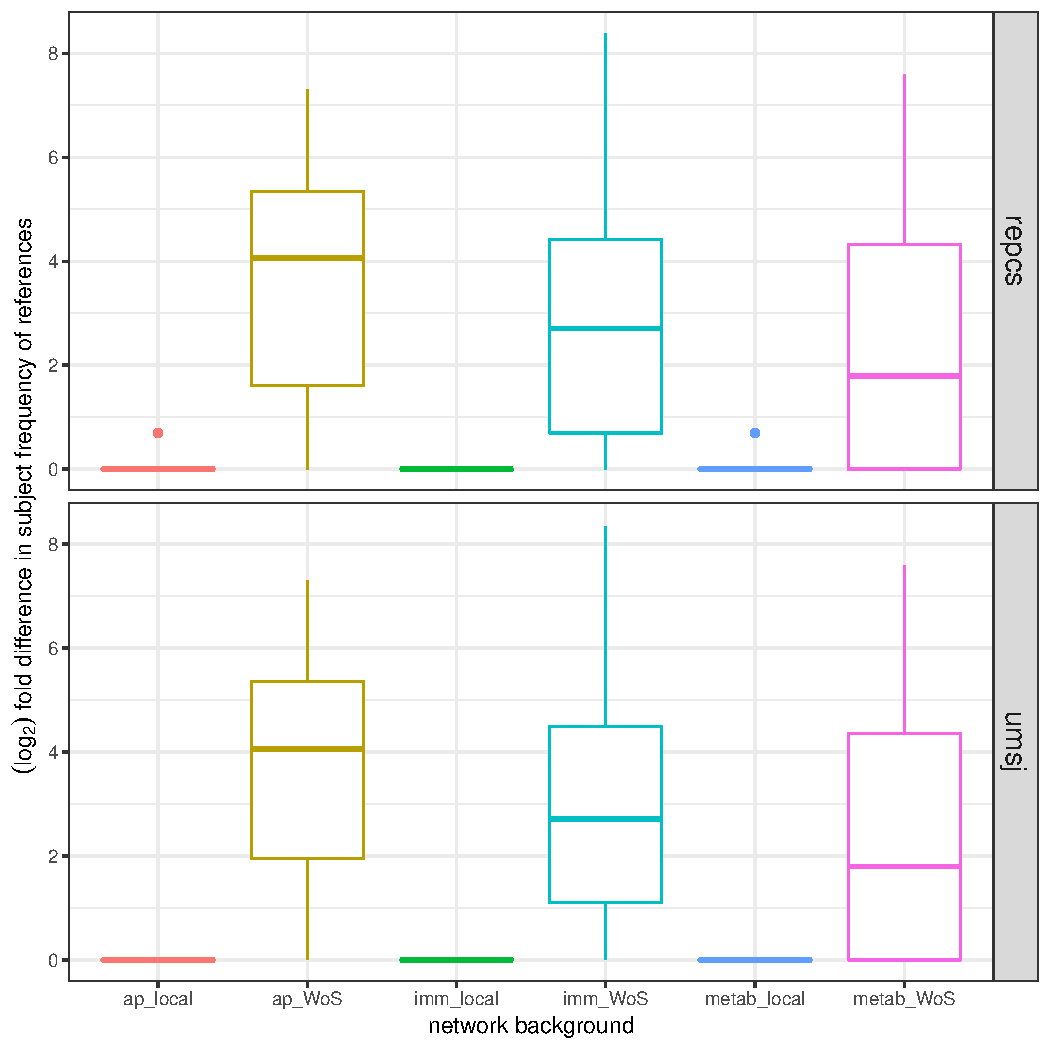
\includegraphics[width=0.8\linewidth]{background-effect}     
\caption{\ Intra-network citation shuffling preserves the disciplinary composition of references. Publications of type Article belonging to the three disciplinary networks (i) Applied Physics (ii) Immunology (iii) Metabolism were subject to a single shuffle of all their cited references using either the cited references in these networks as a source of random substitutions (bg\_local) or references from all articles in WoS (bg\_allWoS). Citation shuffling was performed using either our algorithm (repcs) or that of Uzzi (umsj). The disciplinary composition of cited references before and after shuffling was measured as frequencies for each of 153 sub-disciplines (from the extended subject classification in WoS) and expressed as fold difference between citation counts grouped by subject for original (o) and shuffled (s) references using the formula (fold\_difference = $ifelse(o > s, o/s, s/o)$) and rounded to the nearest integer. Null values were set to 1. A fold difference of 1 indicates that citation shuffling did not alter disciplinary composition. Data are shown for articles published in 1985. All four boxplots are generated from 151 observations. Min \& Max values for fold differences were as follows. (i) Arts \& Humanities. bg\_local (1,2), bg\_allWoS (1, 488) (ii) Life Sciences \& Biomedicine. bg\_local(1,1), bg\_allWos (1, 352) Note y-axis: $log_2$ scale.} 
\label{fig:be}
\end{figure}

Figure \ref{fig:scatter} shows that the z-scores for the same journal pair can be positive (negative) when computed with respect to one data set but be negative (positive) for another data set. The journal-pair z-scores in Figure \ref{fig:scatter} have consistent signs for both Immunology and WoS data sets in 71.4\% of the instances and different signs for 28.6\% of the journal pairs. When a journal-pair z-score is negative with respect to one dataset and positive with respect to another dataset, articles citing that pair are more likely to be deemed novel in the first instance and less likely to be deemed novel in the second instance.  It seems that any journal pair should either be indicative of novelty or not, but it should never have contradictory implications that depend on the reference dataset. We view, therefore, these contradictions as symptomatic of inappropriately sampling from a broad dataset and ignoring observed citation patterns.  Figure \ref{fig:scatter} reflects that the WoS data set has approximately 44,000 fewer negative z-scores than does the immunology data set, which contributes to its significantly lower percentage of high-novelty articles.  \emph{The plots I made of the cumulative z-score distributions for Immunology and WoS also could be used to demonstrate this phenomenon, although the scatter plot does this more clearly, and it is more striking.  The scatter plot also encodes more data, that is, the matched z-scores for each journal pair.}

Note also in Figure \ref{fig:scatter} that many z-scores values are significantly different between the WoS and Immunology datasets, although the density of points near the origin in Figure \ref{fig:scatter} indicates that some journal pairs change signs between the datasets while their magnitudes are not significantly different. While no metric is without downside, this observation points to a weakness of measuring novelty based simply on the sign of z-scores where no distinction is made between a small negative value and a large negative value, but a negative value of small magnitude is viewed as being significantly different than a small positive value.


\begin{figure}%[tbhp]
\centering
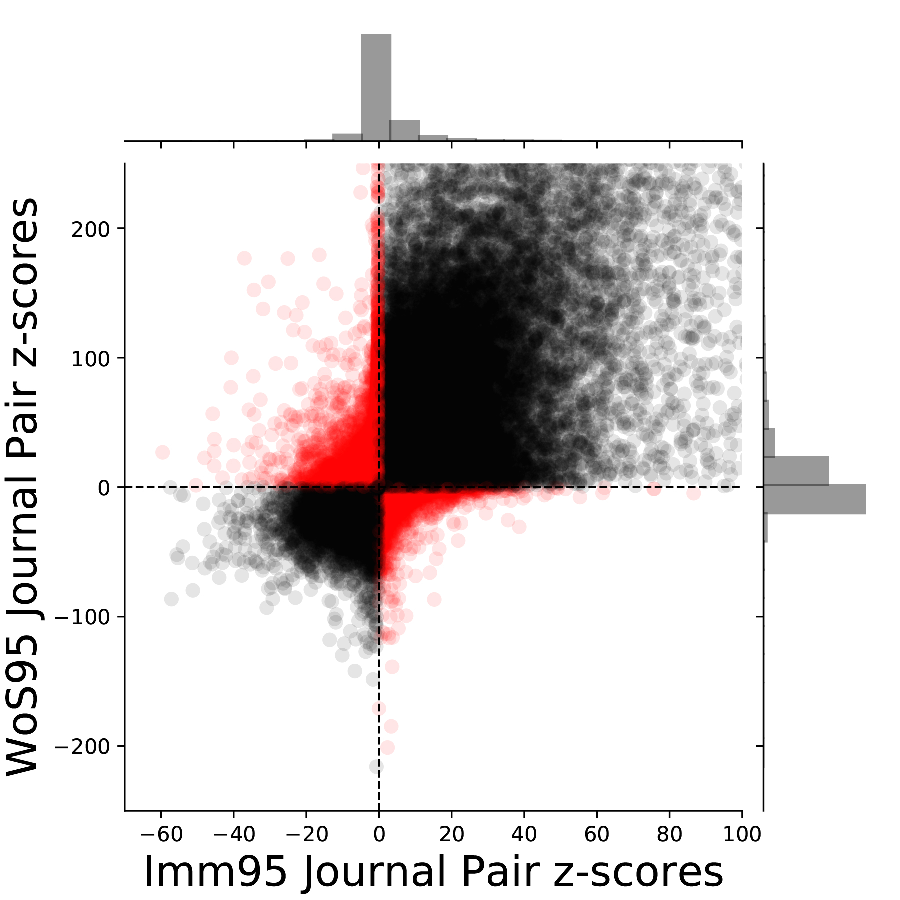
\includegraphics[width=3in]{fig2_scatter_z_scores_flattened.pdf}     %width=.8\linewidth
\caption{Journal pair z-scores vary with reference dataset. Scatter plot points (319,005) indicate journal pair z-scores for the 1995 Immunology dataset along the x-axis and the 1995 Web of Science dataset on the y-axis. Black indicates journal pairs whose z-scores have the same sign when computed for both reference datasets while red points indicate the 28.6\% of journal pairs whose z-scores change sign across datasets. Regions with deeper hues indicate higher point densities and the histograms show the marginal distributions for each dataset separately.}
\label{fig:scatter}
\end{figure}

%\begin{figure*}
%\begin{tabular}{ccc}
%\includegraphics[width=2.1in]{SIDoc/figs/scatter_z_scores_metab85_WoS_ZoomIn.pdf} & 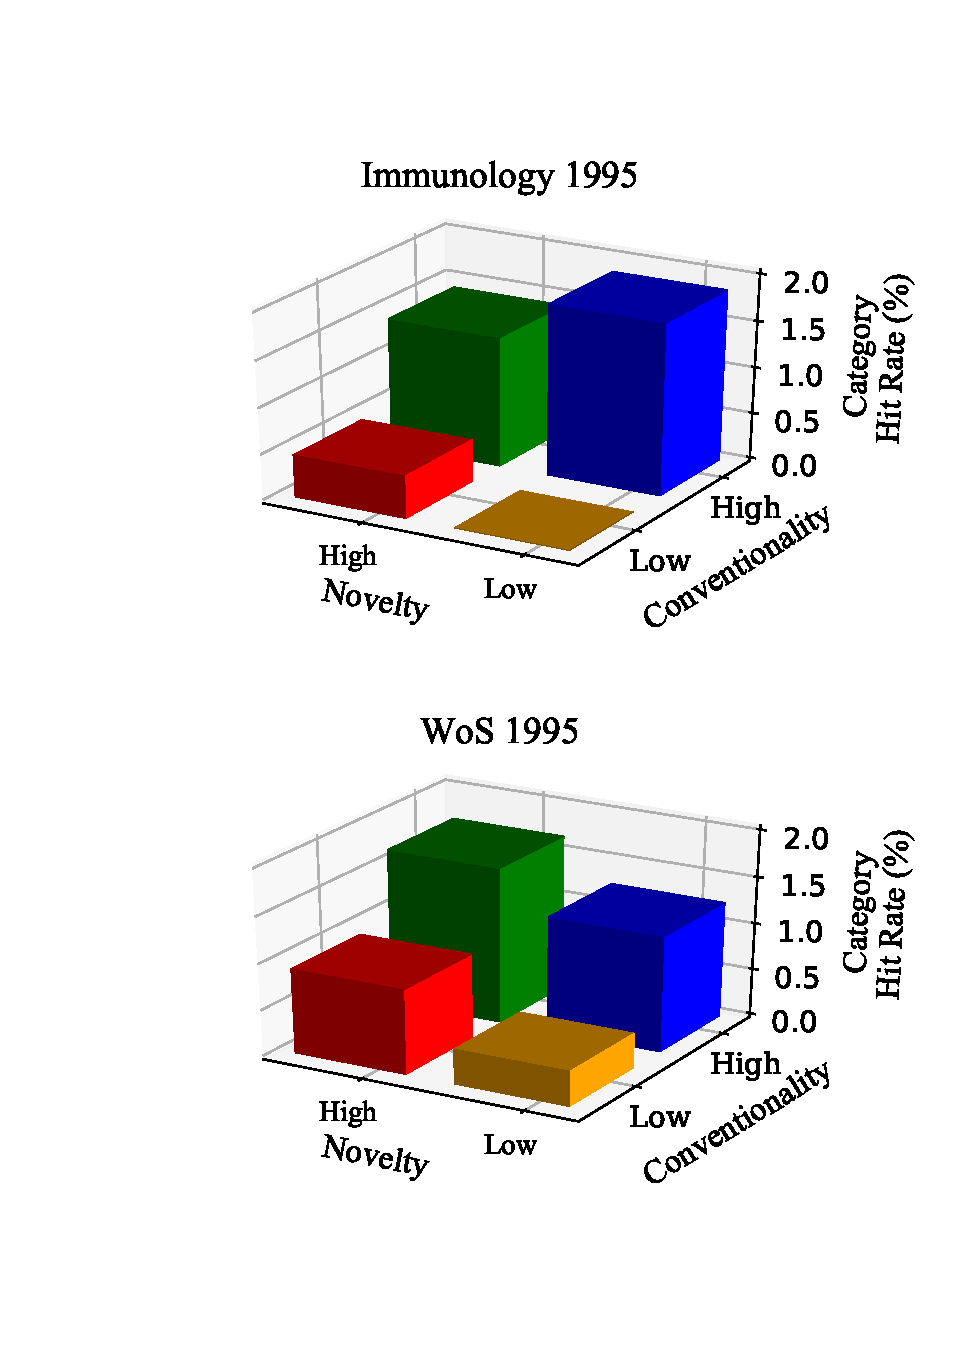
\includegraphics[width=2.1in]{Fig2H01N10.pdf} & 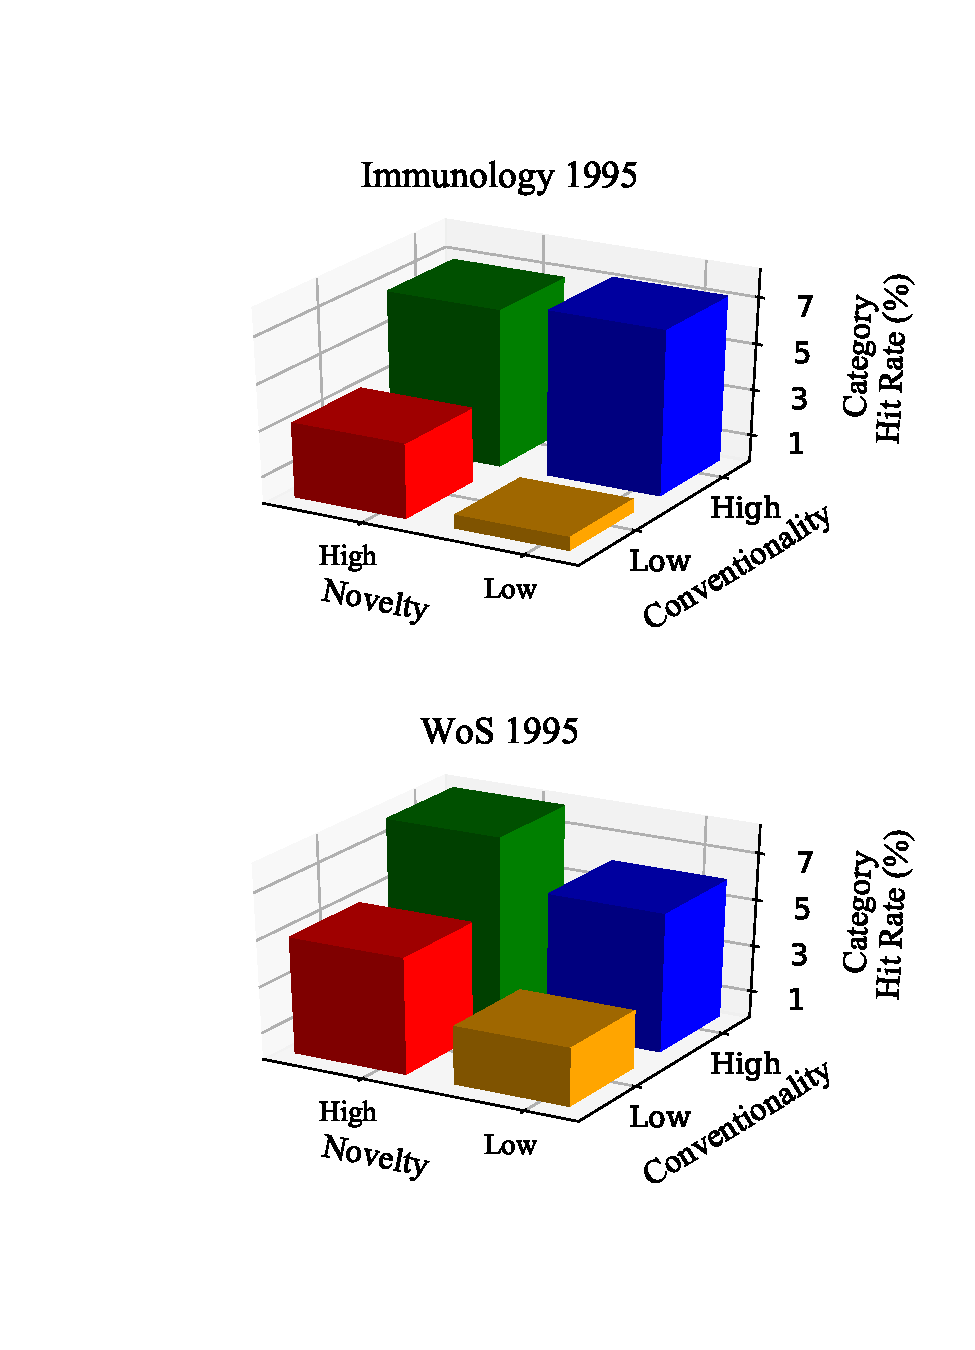
\includegraphics[width=2.1in]{Fig2H05N10.pdf} \\
%(a) & (b) & (c) \\
%\end{tabular}
%\caption{Scatter plot points show journal pair z-scores with respect to the Immunology data set for 1995 on the x-axis and the broad Web of Science on the y-axis. Black indicates journal pairs whose z-scores have the same sign when computed for both data sets while red points indicate journal pairs whose z-scores change sign across data sets. Regions with deeper hues indicate higher point density. The histograms show the marginal distributions of the z-scores for each of the data sets separately.}
%\label{fig:Fig2}
%\end{figure*}

The variation in z-scores with respect to the reference datasets causes the percentages of articles denoted as highly conventional and highly novel to be significantly different, as demonstrated in Figure \ref{fig:Fig1}. \emph{Insert text about Figure \ref{fig:Fig1}.}

\begin{figure}
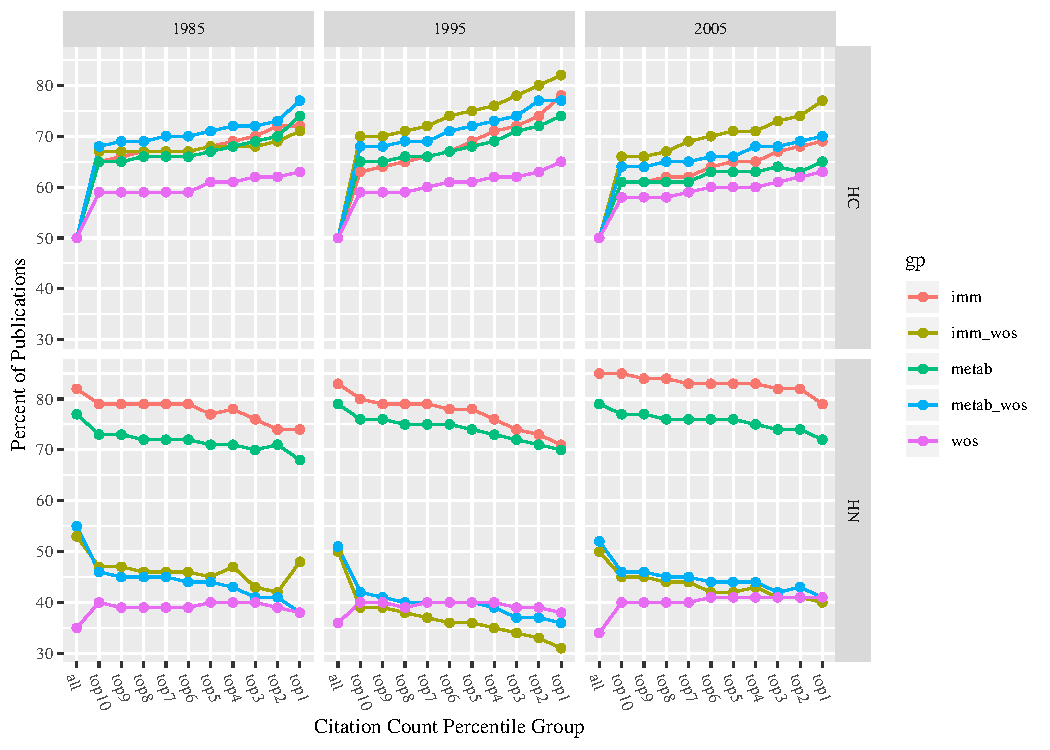
\includegraphics[width=\hsize]{Fig1}
\caption{Fraction of publications with high conventionality (HC) and high novelty (HN) signatures relative to citation count.      \emph{What follows is the caption from PNAS submission: is any of this useful?}  Effect of Research Discipline,  Background Network,  and Citation Count on Conventionality and Novelty.
Data are shown for the applied physics (18,305), immunology (21,917), metabolism (97,405) and WoS (476,288) networks for 1995. The number of publications in each network is shown in parentheses. Citation counts shown are cumulative over the first 8 years since publication. 
X-axis: publications were classified into percentile groups based on citation counts (e.g., Top 1 indicates those publications in the top 1\%). Y axis: The percent of applications in each group that are high conventionality (HC) and high novelty (HN). The z-scores are computed for each disciplinary network based on the selected background network; thus, \emph{imm} denotes the immunology network with immunology z-scores and \emph{imm\_wos} denotes the immunology network with z-scores from WoS z-scores. The figure shows striking differences between the WOS network compared to the metabolism and immunology networks: across all networks, the percentage of high conventionality (HC) publications increases with citation counts, while the percentage of high novelty (HN) publications decreases with citation counts for the biological networks but not for WOS. \label{fig:Fig1}}
\end{figure}

Another symptom of model misspecification is that random sampling of citations associated with an article do not match with the distribution of citations across the disciplines observed in articles from that discipline. \citep{wallace_lariviere_gingras_2012} found that, often, a majority of an article's citations are from the specialty of the article, although that percentage varied among disciplines in the eight specialties they investigated: from approximately 39\% to 89\% for 2006. \emph{More needed here.}  Similarly, we found that 77.4\% of citations in applied physics articles in 1985 (replace with 1995 data?) were from applied physics.  \emph{Add references to other datasets.} A random sampling of citations would ideally reflect the percentages from the discipline in question, as well as the percentages of articles from other disciplines.

We investigated the effect of sampling from disciplinary data sets versus more broadly from the WoS on the disciplinary make-up of the citations in articles under random sampling (\emph{sentence needs work but is an example of a transition.}) \emph{Insert text about Figure \ref{fold_effect}, specifically the right-hand side of Figure  \ref{fold_effect} where the fold statistics demonstrate the effect with Uzzi's approach.} 

\emph{Insert comment about the left-hand side of Figure \ref{fold_effect} where the disciplinary dataset has resolved the fold issue.}  We also predicted that model misspecification as measured by the Kullback-Leibler (K-L) Divergence~\citep{kullback_information_1951} between observed and simulated frequencies in a disciplinary network would be less than the divergence for observed and simulated frequencies in the WoS superset. The results in Table \ref{tab:kld} indicate that for the set of journals common to both a disciplinary network and the WoS superset, simulations under our model consistently have a lower K-L divergence compared to simulations that draw from the WoS superset (and its attendant substitutions that are ectopic with respect to field and discipline).


\begin{table}[ht]
\caption{Measuring Model Misspecification. For the set of journal pairs in common between a disciplinary network and the full WoS dataset, Kullback-Leibler (K-L) divergences
between empirical and simulated journal pair frequencies were computed for the years 1985, 1995, and 2005 for the three disciplinary datasets (applied\_physics, immunology, and metabolism) using either the disciplinary network as background or the WoS superset (all\_wos) to generate the null model (Background). K-L divergence was calculated using the R seewave package with a base (logarithm) of 2. The ratio between the K-L divergence for disciplinary networks versus the full WoS ranges from 1.96 to 2.77 and is greater than 2.0 for eight out of nine cases, strongly suggesting that simulations that constrain substitutions to the given disciplinary network better model the observed data.}
\label{tab:kld}
\centering
\begin{tabular}{|r lrlr r|}
  \hline
 & Disciplinary Network & Year & Background & K-L Divergence & Ratio \\ 
  \hline
1 & appl\_physics & 1985 & appl\_physics & 1.21 &  \\ 
  2 &  & 1985 & all\_wos & 2.37 & 1.96 \\ 
  3 &  & 1995 & appl\_physics & 0.86 &  \\ 
  4 &  & 1995 & all\_wos & 2.37 & 2.77 \\ 
  5 &  & 2005 & appl\_physics & 0.95 &  \\ 
  6 &  & 2005 & all\_wos & 2.35 & 2.47 \\ 
    \hline
  7 & immunology & 1985 & immunology & 0.75 &  \\ 
  8 &  & 1985 & all\_wos & 1.68 & 2.24 \\ 
  9 &  & 1995 & immunology & 0.78 &  \\ 
  10 &  & 1995 & all\_wos & 1.70 & 2.19 \\ 
  11 &  & 2005 & immunology & 0.73 &  \\ 
  12 &  & 2005 & all\_wos & 1.92 & 2.63 \\ 
    \hline
  13 & metabolism & 1985 & metabolism & 1.11 &  \\ 
  14 &  & 1985 & all\_wos & 2.24 & 2.02 \\ 
  15 &  & 1995 & metabolism & 1.07 &  \\ 
  16 &  & 1995 & all\_wos & 2.33 & 2.17 \\ 
  17 &  & 2005 & metabolism & 1.19 &  \\ 
  18 &  & 2005 & all\_wos & 2.60 & 2.18 \\ 
   \hline
\end{tabular}
\end{table}



\subsection{Novelty and Conventionality as Determinants of Impact in Disciplinary Contexts}


\begin{figure*}
\centering
\begin{tabular}{ccc}
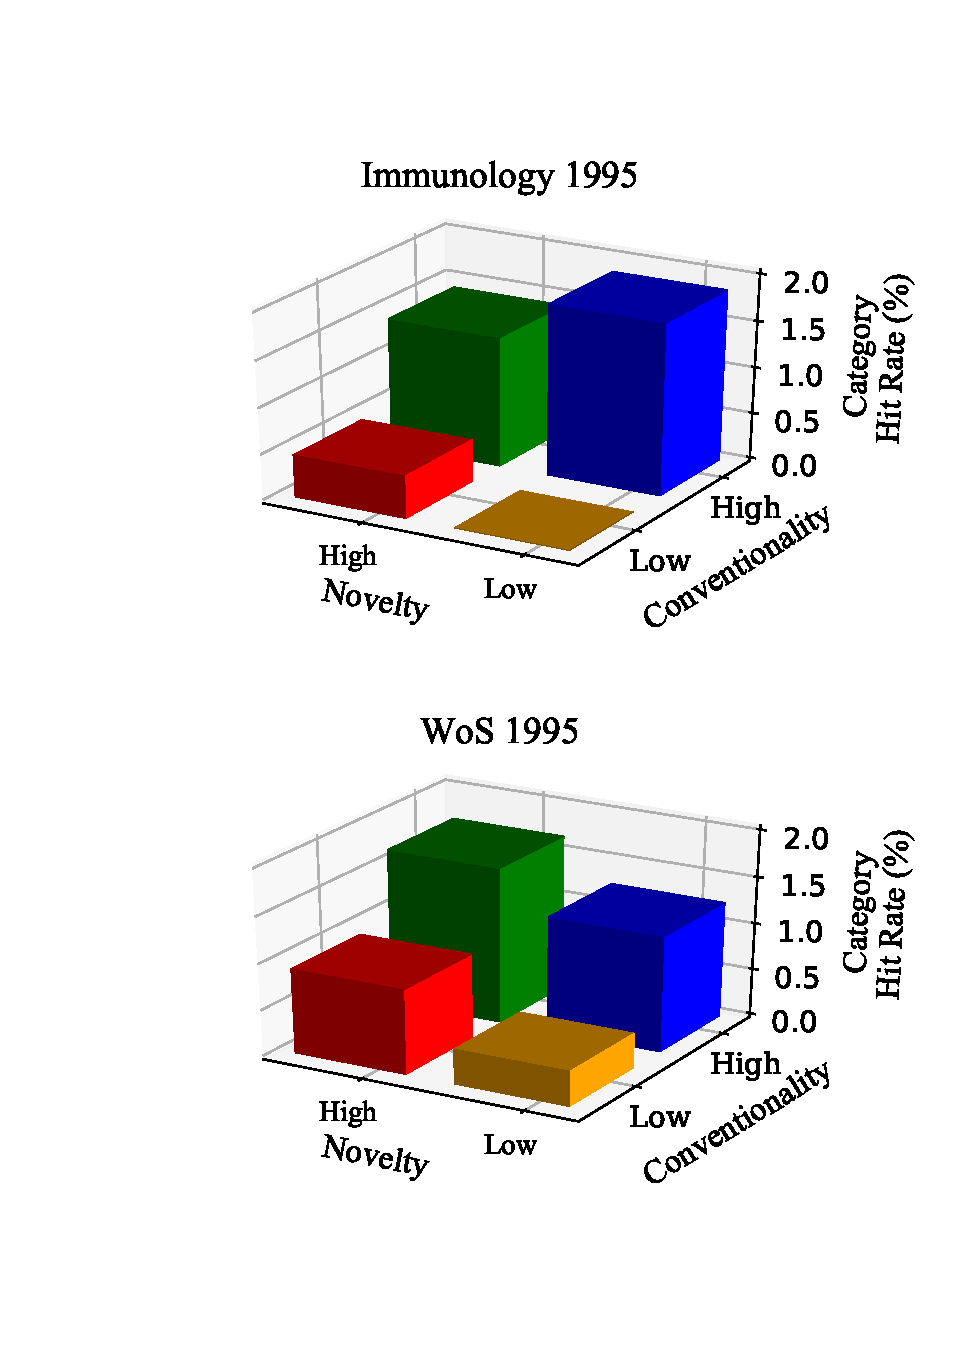
\includegraphics[width=1.5in]{Fig2H01N10.pdf} & 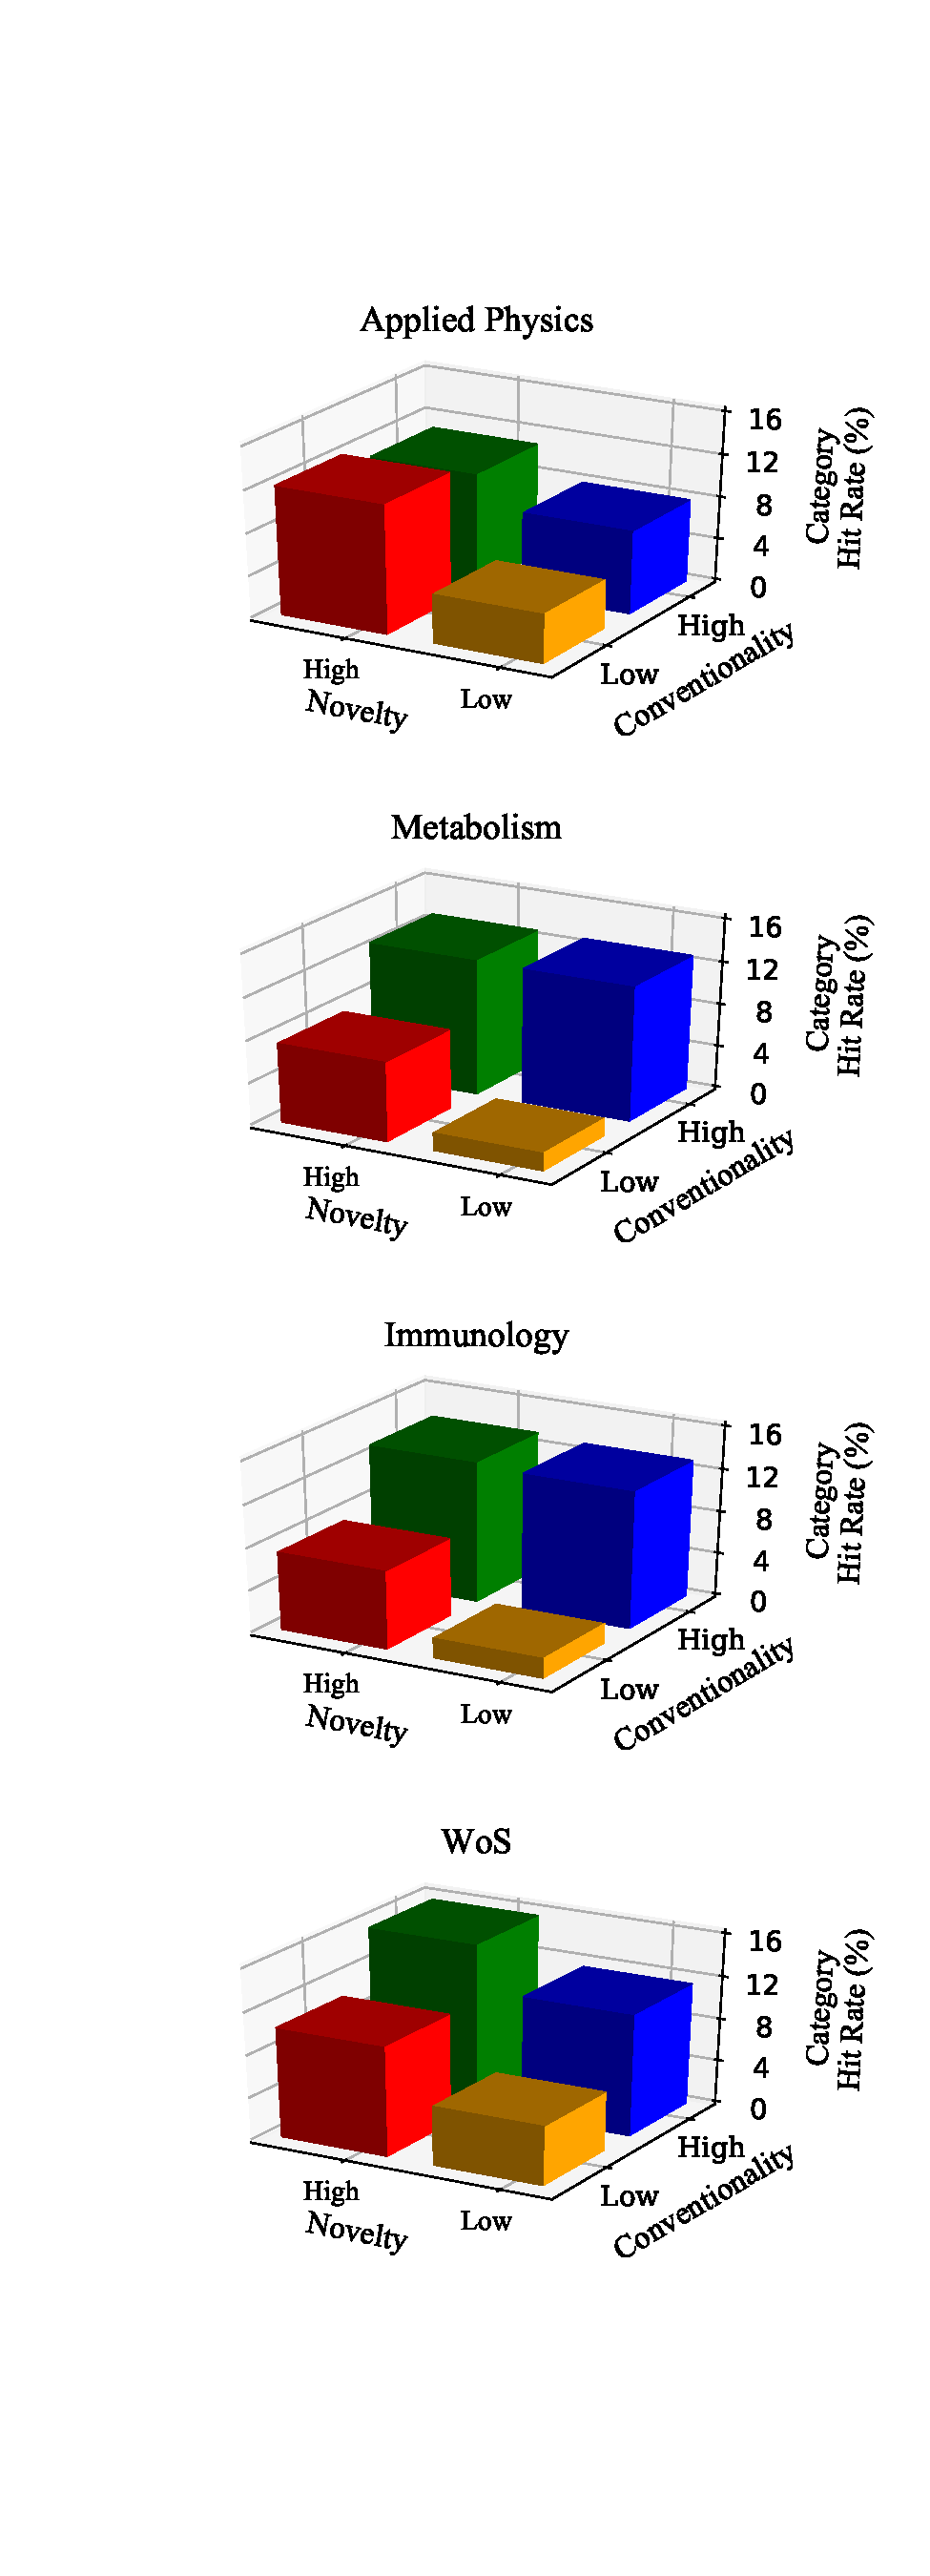
\includegraphics[width=1.5in]{Fig2H10N10.pdf} \\
(a) & (b) \\
\end{tabular}
\caption{Effect of Context on Journal-Pair z-scores and Categorical Hit Rates: Immunology, Applied Physics, and WoS for 1995. Panels (a) and (b) show hit rates for the LNLC, LNHC, HNLC, and HNHC categories for the immunology, applied physics, and WoS datasets when hit articles are defined as the top 1\% and top 10\% of articles, respectively.  Novelty in both panels is defined at the 10th percentile of articles' z-score distributions. The number of data points in the immunology, applied physics, and WoS data sets are 21,917, 18,305, and 476,288, respectively.  The results for the WoS data set mirrored previous results from Uzzi et al. ~\cite{uzzi_atypical_2013} where the highest hit rate was for the HNHC category.  The highest hit rates for the immunology dataset, in contrast, are in the LNHC category. The LNHC category often had the highest hit rate for the immunology dataset for various parameter settings with the HCHN category having the highest hit rate in other cases: metabolism results are similar. The applied physics dataset shows further contrast as the hit rate for it was highest in the HNLC category.  The HNLC category demonstrated the highest hit rate often for applied physics: otherwise the highest hit rate was for HNHC articles.}
\label{fig:Fig2}
\end{figure*}


Figure \ref{fig:Fig2}, Panels (a) and (b), compares hit rates for the four categories among the Immunology, Applied Physics, and WoS datasets for 1995: the hit rate is defined as the number of hit articles in each category divided by the number of articles in the category. We evaluated the statistical significance of the categorical hit rates using multiple methods, some of which we describe here.  Our first test was based on the null hypotheses that hits were distributed randomly among the four categories with uniform probability in proportion to the number of articles in each category. Using a Chi-Square Goodness of Fit test, rejecting the null hypothesis in favor of the alternate hypothesis supports a non-uniform dispersion of hits: that is, some of the four categories are individually associated with higher than expected, or lower than expected hit rates. The null hypothesis was rejected at a $p<0.001$ in all cases in  Figure \ref{fig:Fig2}, with the exception of the immunology and applied datasets where hit articles are designated as the top 1\% of articles: valid tests were not possible in those instances due to too few expected hits. The null hypothesis was rejected with $p<0.001$ for all valid tests for all parameter settings, all datasets, and all years: hypotheses tests were valid in 73 of 96 instances. We conclude that it is likely that the distribution of hits among categories is not uniform but, rather, hit rates vary among the categories in all datasets. (Should we insert a table with all statistical results?)


\begin{table}%[tbhp]
\centering
\caption[Hit Rates]{Hit Rates by Category. The last four columns indicate the proportion of publications that are hits for each respective category.} \label{Tab:HitRate}
\begin{tabular}{crrrrrrr}
& \multicolumn{1}{c}{Hits as \%} & \multicolumn{1}{c}{Novelty}  &  &  &  &  \\ Data Set & \multicolumn{1}{c}{of Articles} & \multicolumn{1}{c}{Percentile} & \multicolumn{1}{c}{LNLC} & \multicolumn{1}{c}{LNHC} & \multicolumn{1}{c}{HNLC} & \multicolumn{1}{c}{HNHC} \\ \hline
   
Imm95&1\%&10\%& 0.000& 0.019& 0.005& 0.014 \\ 
Imm95&10\%&10\%& 0.017& 0.128& 0.076& 0.129 \\ 
Metab95&1\%&10\%& 0.001& 0.017& 0.006& 0.014 \\ 
Metab95&10\%&10\%& 0.019& 0.130& 0.074& 0.133 \\ 
AP95&1\%&10\%& 0.002& 0.007& 0.012& 0.010 \\ 
AP95&10\%&10\%& 0.047& 0.079& 0.123& 0.109 \\ 
WoS95&1\%&10\%& 0.004& 0.013& 0.009& 0.017 \\ 
WoS95&10\%&10\%& 0.056& 0.115& 0.104& 0.156 \\ \hline

\end{tabular}
\end{table}


We computed hit rates for the WoS dataset, which mirrored Uzzi et al.'s results whereby the largest hit rates were for the HNHC category, despite our methodological improvement of sampling citations in proportion to their frequency. We found contrary results in the 1995 immunology dataset where articles in the LNHC category often had the greatest hit rates, as reflected in Table \ref{Tab:HitRate} and Figure \ref{fig:Fig2}.  Across all year's data, all datasets, and all parameter settings, the highest hit rates in the immunology datasets were sometimes in the LNHC category and sometimes in the HNHC category. The metabolism hit rates reflected this same pattern. The greatest hit rates for the applied physics data were often in the HNLC category as reflected in Table \ref{Tab:HitRate} and Figure \ref{fig:Fig2}, and otherwise in the HNHC category. We conclude that Uzzi et al.'s finding of high hit rates in the HNHC category does not hold generally for disciplinary-based datasets and that novel citation patterns are not always indicative of impactful research, as was the case with immunology. Furthermore, the categories displaying the greatest hit rate vary with parameter settings and with the year. The lack of stable results across parameter settings suggests that parameters must be selected judiciously.

We also tested the explanatory power of each framework dimension by classifying articles as Low Novelty (LN) or High Novelty (HN) and, separately, as having Low Conventionality (LC) or High Conventionality (HC).  We tested the null hypothesis that hits are distributed between LN and HN (LC and HC) in proportion to the total number of articles assigned to those categories.  That null hypothesis was rejected for the WoS data along both dimensions. Consistent with previous analysis, hit articles were overrepresented in the HC category in every instance of WoS data at a $p<0.001$ and hit articles were overrepresented in the HN category at a $p<0.001$ in all but two cases.  The p-values, in those cases, were 0.002 and 0.007.  Hits in the immunology and metabolism data were overrepresented in the HC category with the same statistical significance as for WoS. The relationship of novelty with hits in the immunology and metabolism data differed dramatically from the WoS, however, with statistically significant findings of hit articles being sometimes overrepresented in the LN category, and sometimes being underrepresented.  Of the 12 tests for applied physics, the statistical significance supporting a positive relationship between hit articles and HN were all $p<0.10$, and 10 of 12 were $p<0.05$.  These tests also indicated strong support for the relationship between LN and hit articles in applied physics in a limited number of tests, with $p<0.10$ in 5 of 12 instances and $p < 0.05$ in 3 of 12 instances. These results suggest that (1) both conventionality and novelty are strongly related to hits in the WoS, (2) the conventionality dimension is strongly related with hits in immunology and metabolism and novelty is not, (3) novelty is more strongly related with hits in applied physics than is conventionality. More generally, we find that the dimensions most strongly related with hit articles vary across disciplines and between disciplinary and broad data sets. 


\section{Discussion}

We conclude that Uzzi et al.'s finding of high hit rates in the HNHC category does not hold generally for all datasets and that novel citation patterns are not always indicative of impactful research.

The z-scores that change sign across datasets is either contradictory or an acceptable variation due to the difference in reference sets. We contend that it is the former because the inappropriate substitution of citations with those from disciplines that are implausible and because the observed citation frequencies are ignored. That fewer z-scores are negative in the WoS dataset relative to the immunology dataset may be directly due to the uniform sampling of references whereby many resulting journal pairs are never observed in the literature and so that the expected frequencies of those observed pairs have lower expected values, thus biasing their z-scores upward. In addition, treating citation as a set versus a multiset means that a random model will sample popular citations downward, thus further increasing their z-scores.

Contrary to Uzzi et al. we found the category displaying the highest hit rate to be sensitive to the experimental parameter settings, which included the percentage of articles deemed to be hits and the percentile of articles' z-score distributions that delineated between articles of low novelty and high novelty. Faced with this lack of robustness, we are confronted with the necessity of defining defendable parameters, if possible, that determine novelty and conventionalty. More significantly, we should question whether the simple approach of defining novelty and conventionality as is done this article and other research is sufficient or whether we should expect such variation in the factors associated with impact as we have observed.

George's point from Slack conversation: ``A concern that surfaced on the drive are the definitions of conventionality and novelty. On the one hand we use them- on the other hand you've also pointed out that it isn't that simple.''

\acknowledgments
We are grateful to Kevin Boyack and Dick Klavans for constructively critical discussions. We thank the authors of Uzzi et al. (2013) for sharing their Python simulation code. Research and development reported in this publication was partially supported by Federal funds from the National Institute on Drug Abuse, National Institutes of Health, US Department of Health and Human Services, under Contract Nos. HHSN271201700053C (N43DA-17-1216) and HHSN271201800040C (N44DA-18-1216). The content of this publication is solely the responsibility of the authors and does not necessarily represent the official views of the National Institutes of Health. TW receives funding from the Grainger Foundation. All the code used in this study is freely available from a Github site. Access to the bibliographic data analyzed in this study requires a license from Clarivate Analytics, which had no role in funding, experimental design, review of results, and conclusions presented. 

\authorcontributions 
This study was designed by GC, JB, SD, and TW. Simulations and analysis were performed by AD, GC, JB, and SD. Infrastructure and workflows used to generate data used in this study were developed by AD, DK, SL, SD, and GC.  All authors reviewed and commented on the manuscript, which was written by GC, JB, and TW.

\newpage
%%%%%%%%%%%%%%%%%%%%%%%
%% The bibliography

\bibliography{cocit_r}

%% No appendices allowed in Network Neuroscience style
%\appendix

\end{document}

\subsection{Sample Subsection}
Text here. Text here. Text here. Text here.
Text here. Text here. Text here. Text here.
Text here. Text here. Text here. Text here.
Text here. Text here. Text here. Text here.

\subsubsection{Sample Subsubsection}
Text here. Text here. Text here. Text here.
Text here. Text here. Text here. Text here.
Text here. Text here. Text here. Text here.
Text here. Text here. Text here. Text here.


\section{Sample equations}
\begin{equation}
\label{eq:rhoCHT}
\rho^{\pi}= \frac{RI + \mathbb{E}_{\pi([L,\tau_L]|\textrm{post})}
\left[C_L(\taupav+\tau_L) \right]   +
\displaystyle{\int_{0}^{P}}{dw~ \mathbb{E}_{\pi_{w_L}}}
\Biggl[\/\sum_{n_{L|[\textrm{pre},w]}}C_L(\tau_L)
\Biggr]            }      {P +
\mathbb{E}_{\pi([L,\tau_L] |\textrm{post})}[\tau_{L}] +\taupav +
\displaystyle{ \int_{0}^{P}}{dw~ \mathbb{E}_{\pi_{w_L}}}   
\Biggl[\sum_{n_{L|[\textrm{pre},w]}}\tau_L\Biggr]  
}
\end{equation}
As long as
$RI - K_LP > 
\frac{1}{\beta}$
\begin{equation}
%\def\theequation{5.1}
\left.\begin{array}{lrcl}
&\rho^{\pi} &=&  \displaystyle\frac{\beta ( RI + K_L \taupav )-1} {\beta
(P+\taupav )}    \\[12pt]
\hbox{and}\hbox to .25in{\hfill}&\mathbb{E}[\tau_L | \text{post}] &=&\displaystyle \frac{P+\taupav}{\beta ( RI -
K_LP)-1}  
\label{eq:analytical_linear}
\end{array}\right\}\hbox to 1.25in{\hfill}
\end{equation} 
Text finishing first page.
Text finishing first page.
Text finishing first page.
Text finishing first page.
Text finishing first page.
Text finishing first page.
Text finishing first page.


\begin{boxedtext}{Comparative Analysis of Different Classes of Networks} 
Going beyond the examination of shared topological features across
nervous systems, the generalized mathematical language of graph theory
also offers tools for the comparison of the organization of brain
networks to other classes of network studied
by different scientific
disciplines. 

Many real-world systems operate as some sort of
interaction or communication network, including, for example, social
networks, gene regulatory networks, computer networks, and
transportation networks. Similar to brain networks, many of these
real-world networks display an efficient small-world organization, a
pronounced community structure with densely connected modules, as well
as the formation of hubs and rich clubs. Going beyond the
comparison of networks within the class of nervous systems, the field
of `comparative network analysis' examines commonalities and
differences across a range of network classes.

\begin{figure}
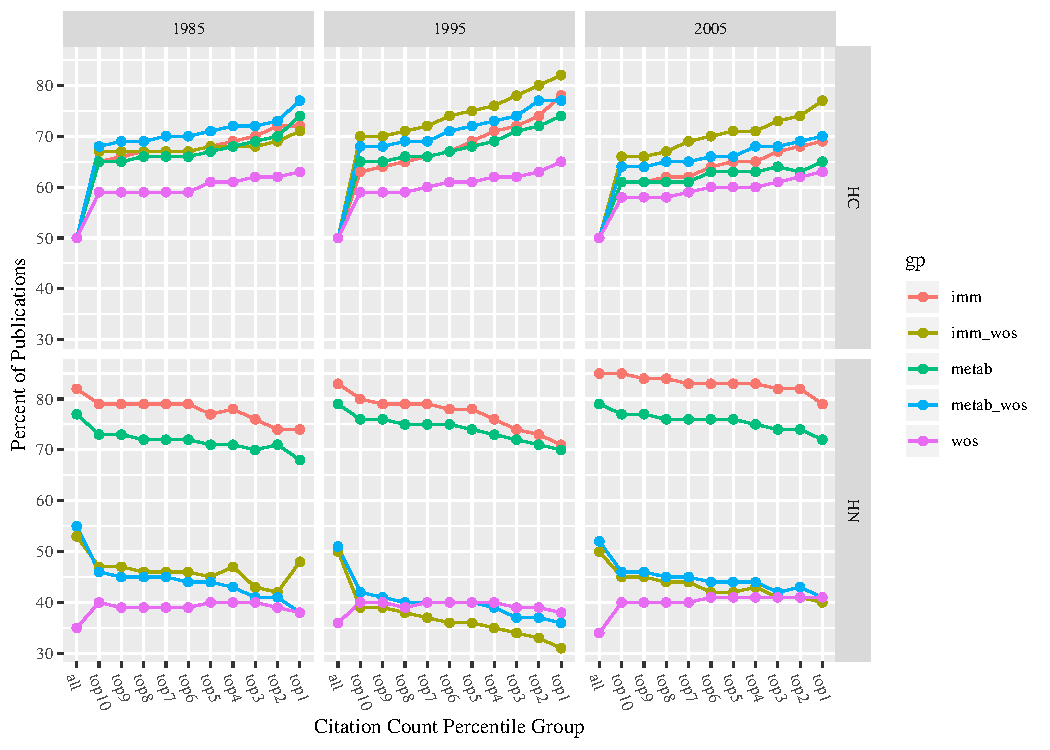
\includegraphics[width=\hsize]{Fig1}
\caption{Here is the caption.}
\end{figure}
\end{boxedtext}

\newpage
\begin{boxedtext}{Comparative Analysis of Different Classes of Networks} 
Going beyond the examination of shared topological features across
nervous systems, the generalized mathematical language of graph theory
also offers tools for the comparison of the organization of brain
networks to other classes of network studied by different scientific
disciplines. Many real-world systems operate as some sort of
interaction or communication network, including, for example, social
networks, gene regulatory networks, computer networks, and
transportation networks. Similar to brain networks, many of these
real-world networks display an efficient small-world organization, a
pronounced community structure with densely connected modules, as well
as the formation of hubs and rich clubs. Going beyond the
comparison of networks within the class of nervous systems, the field
of `comparative network analysis' examines commonalities and
differences across a range of network classes.

\begin{table}[ht]
\caption{Here is the caption.}

\centerline{\begin{tabular}{|c|c|c|}
\hline
one&two&three\\
\hline
four&five&six\\
\hline
\end{tabular}}
\end{table}
\end{boxedtext}

\subsection{Jargon Samples in margin}
One common decision is between working (performing an employer-defined
task) and engaging in leisure (activities pursued for oneself). Working
leads to external rewards such as food and money; whereas leisure is
supposed to be intrinsically beneficial \jargon{Intrinsically beneficial}{The characteristic of
leisure that we enjoy most.} (otherwise one would not want to
engage in it).
%% \jargon has optional argument in square brackets where you can specify
%% the amount of extra space below where it would normally appear when 
%% two \jargon entries are in the same paragraph:
$\beta \in [0,\infty)$\jargon[24pt]{$\beta \in [0,\infty)$}{inverse temperature or degree of
stochasticity-determinism parameter.} is often used to indicate an
important parameter, the stochasticity-determinism parameter.

\subsection{Simple code sample}

\begin{code}
\begin{verbatim}
procedure bubbleSort( A : list of sortable items )
    n = length(A)
    repeat
       newn = 0
       for i = 1 to n-1 inclusive do
          if A[i-1] > A[i] then
             swap(A[i-1], A[i])
             newn = i
          end if
       end for
       n = newn
    until n = 0
end procedure
\end{verbatim}
\end{code}


\subsection{Algorithm environment}
%% \begin{algorithm} takes option [p][b][t][h],  or some combination, like \begin{figure}
%% See documentation for algorithmic.sty for more information on formatting algorithms.

\begin{algorithm}[h]
\caption{A sample in an algorithm environment.}
\begin{algorithmic}
\If {$i\geq maxval$}
    \State $i\gets 0$
\Else
    \If {$i+k\leq maxval$}
        \State $i\gets i+k$
    \EndIf
\EndIf
\end{algorithmic}
\end{algorithm}


\section{Itemized Lists}

\subsection{Roman list:}

\begin{enumerate}
\item[(i)] at high 
payoffs, subjects work almost continuously.
\item[(ii)] at low payoffs, they 
engage in leisure all at once, in long bouts after working.
\item[(iii)] subjects work continuously for the entire price duration, as long as
the price is not very long;
\item[(iv)] the duration of leisure bouts is variable.
\end{enumerate}


\subsection{Numbered list:}

\begin{enumerate}
\item at high 
payoffs, subjects work almost continuously, engaging in little leisure
inbetween work bouts; 
\item at low payoffs, they 
engage in leisure all at once, in long bouts after working, rather
than distributing the same amount of leisure time into multiple short
leisure bouts; 
\item subjects work continuously for the entire price duration, as long as
the price is not very long (as shown by an analysis conducted by
Y-AB, to be published separately);  
\item the duration of leisure bouts is variable.
\end{enumerate}


\subsection{Bulleted list:}

\begin{itemize}
\item at high 
payoffs, subjects work almost continuously, engaging in little leisure
inbetween work bouts; 
\item at low payoffs, they 
engage in leisure all at once, in long bouts after working, rather
than distributing the same amount of leisure time into multiple short
leisure bouts; 
\item subjects work continuously for the entire price duration, as long as
the price is not very long (as shown by an analysis conducted by
Y-AB, to be published separately);  
\item the duration of leisure bouts is variable.
\end{itemize}

\subsection{Description list:}
\begin{description}
\item[High payoffs:] at high 
payoffs, subjects work almost continuously, engaging in little leisure
inbetween work bouts; 
\item[Low payoffs:] at low payoffs, they 
engage in leisure all at once, in long bouts after working, rather
than distributing the same amount of leisure time into multiple short
leisure bouts; 
\item[Continuous work:] subjects work continuously for the entire price duration, as long as
the price is not very long (as shown by an analysis conducted by Y-AB, to be published separately); 
\item[Duration:] the duration of leisure bouts is variable.
\end{description}


\section{Sample figures}

\begin{figure}[h] 
\centerline{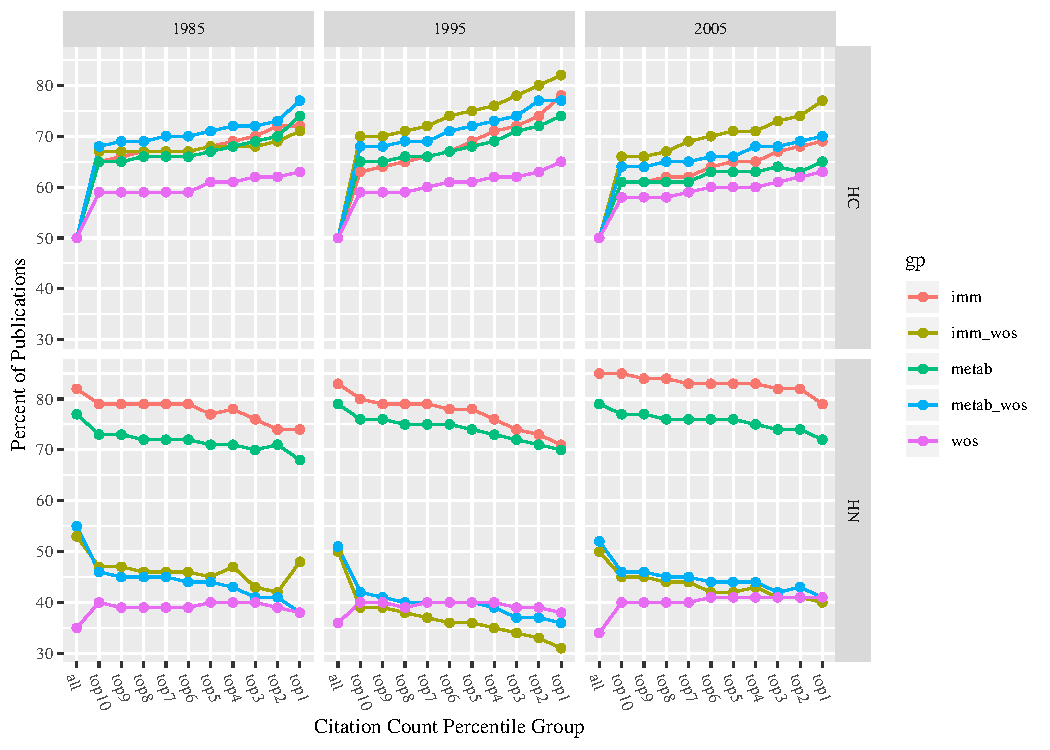
\includegraphics[width=\textwidth]{Fig1.pdf}}
\caption{(Colour online) \textbf{Task and key features of the
 data.} \\
 A) Cumulative handling time (CHT) task. Grey bars denote work
(depressing a lever), white gaps show leisure. The subject must
accumulate work up to a total period of time called the
\emph{price} ($P$) in order to obtain a single reward (black dot) of subjective reward
intensity $RI$. The trial duration is $25\times \mathrm{price}$ (plus
$2$s each time the price is attained, during which the lever is retracted so it cannot
work; not shown).}
\label{fig:task_data}
\end{figure}
%% this command ends a page but does not fill the bottom with white space:
\eject

\begin{figure}[ht] 
\widefigure{\fullpagewidth}{Fig1.pdf}
\caption{(Colour online) \textbf{Task and key features of the
 data.} \\
 A) Cumulative handling time (CHT) task. Grey bars denote work
(depressing a lever), white gaps show leisure. The subject must
accumulate work up to a total period of time called the
\emph{price} ($P$) in order to obtain a single reward (black dot) of subjective reward
intensity $RI$. The trial duration is $25\times \mathrm{price}$ (plus
$2$s each time the price is attained, during which the lever is retracted so it cannot
work; not shown).}
\label{fig:task_data2}
\end{figure}

\newpage
\section{Sample tables}

\begin{table}[!ht]
\caption{Time of the Transition Between Phase 1 and Phase 2$^{a}$}
\label{tab:label}
\centering
\begin{tabular}{lc}
\hline
 Run  & Time (min)  \\
\hline
  $l1$  & 260   \\
  $l2$  & 300   \\
  $l3$  & 340   \\
  $h1$  & 270   \\
  $h2$  & 250   \\
  $h3$  & 380   \\
  $r1$  & 370   \\
  $r2$  & 390   \\
\hline
\multicolumn{2}{l}{$^{a}$Table note text here.}
\end{tabular}
\end{table}

\begin{table}[ht]
\widecaption{Sample table taken from [treu03]\label{tbl-1}}
\begin{widetable}
\advance\tabcolsep-1pt
\small
\begin{tabular}{ccrrccccccccc}
\hline
\bf 
POS &\bf  chip &\multicolumn1c{\bf ID} &\multicolumn1c{\bf X}
&\multicolumn1c{\bf Y} &\bf
RA &\bf DEC &\bf IAU$\pm$ $\delta$ IAU &\bf
IAP1$\pm$ $\delta$ IAP1 &\bf IAP2 $\pm$ $\delta$
IAP2 &\bf star &\bf E &\bf Comment\\
\hline
0 & 2 & 1 & 1370.99 & 57.35\rlap{$^a$}    &   6.651120 &  17.131149 &
21.344$\pm$0.006\rlap{$^b$}  & 2 4.385$\pm$0.016 & 23.528$\pm$0.013 & 0.0 & 9 & -    \\
0 & 2 & 2 & 1476.62 & 8.03     &   6.651480 &  17.129572 & 21.641$\pm$0.005  & 2 3.141$\pm$0.007 & 22.007$\pm$0.004 & 0.0 & 9 & -    \\
0 & 2 & 3 & 1079.62 & 28.92    &   6.652430 &  17.135000 & 23.953$\pm$0.030  & 2 4.890$\pm$0.023 & 24.240$\pm$0.023 & 0.0 & - & -    \\
0 & 2 & 4 & 114.58  & 21.22    &   6.655560 &  17.148020 & 23.801$\pm$0.025  & 2 5.039$\pm$0.026 & 24.112$\pm$0.021 & 0.0 & - & -    \\
0 & 2 & 5 & 46.78   & 19.46    &   6.655800 &  17.148932 & 23.012$\pm$0.012  & 2 3.924$\pm$0.012 & 23.282$\pm$0.011 & 0.0 & - & -    \\
0 & 2 & 6 & 1441.84 & 16.16    &   6.651480 &  17.130072 & 24.393$\pm$0.045  & 2 6.099$\pm$0.062 & 25.119$\pm$0.049 & 0.0 & - & -    \\
0 & 2 & 7 & 205.43  & 3.96     &   6.655520 &  17.146742 & 24.424$\pm$0.032  & 2 5.028$\pm$0.025 & 24.597$\pm$0.027 & 0.0 & - & -    \\
0 & 2 & 8 & 1321.63 & 9.76     &   6.651950 &  17.131672 &
22.189$\pm$0.011  & 2 4.743$\pm$0.021 & 23.298$\pm$0.011 & 0.0 & 4 &
edge \\
\hline\\[-6pt]
\multicolumn{13}{l}{%
Table 2 is published in its entirety in the electronic
edition of the {\it Astrophysical Journal}.}\\[3pt]
\multicolumn{13}{l}{%
$^a$ Sample footnote for table 2.}\\[3pt]
\multicolumn{13}{l}{%
$^b$ Another sample footnote for table 2.}
\end{tabular}
\end{widetable}
\end{table}

\begin{table}[p]
\rotatebox{90}{\vbox{\hsize=\textheight
\caption{Here is a caption for a table that is found in landscape
mode.}
\begin{tabular}{ccrrccccccccc}
\hline
\bf 
POS &\bf  chip &\multicolumn1c{\bf ID} &\multicolumn1c{\bf X}
&\multicolumn1c{\bf Y} &\bf
RA &\bf DEC &\bf IAU$\pm$ $\delta$ IAU &\bf
IAP1$\pm$ $\delta$ IAP1 &\bf IAP2 $\pm$ $\delta$
IAP2 &\bf star &\bf E &\bf Comment\\
\hline
0 & 2 & 1 & 1370.99 & 57.35\rlap{$^a$}    &   6.651120 &  17.131149 &
21.344$\pm$0.006\rlap{$^b$}  & 2 4.385$\pm$0.016 & 23.528$\pm$0.013 & 0.0 & 9 & -    \\
0 & 2 & 2 & 1476.62 & 8.03     &   6.651480 &  17.129572 & 21.641$\pm$0.005  & 2 3.141$\pm$0.007 & 22.007$\pm$0.004 & 0.0 & 9 & -    \\
0 & 2 & 3 & 1079.62 & 28.92    &   6.652430 &  17.135000 & 23.953$\pm$0.030  & 2 4.890$\pm$0.023 & 24.240$\pm$0.023 & 0.0 & - & -    \\
0 & 2 & 4 & 114.58  & 21.22    &   6.655560 &  17.148020 & 23.801$\pm$0.025  & 2 5.039$\pm$0.026 & 24.112$\pm$0.021 & 0.0 & - & -    \\
0 & 2 & 5 & 46.78   & 19.46    &   6.655800 &  17.148932 & 23.012$\pm$0.012  & 2 3.924$\pm$0.012 & 23.282$\pm$0.011 & 0.0 & - & -    \\
0 & 2 & 6 & 1441.84 & 16.16    &   6.651480 &  17.130072 & 24.393$\pm$0.045  & 2 6.099$\pm$0.062 & 25.119$\pm$0.049 & 0.0 & - & -    \\
0 & 2 & 7 & 205.43  & 3.96     &   6.655520 &  17.146742 & 24.424$\pm$0.032  & 2 5.028$\pm$0.025 & 24.597$\pm$0.027 & 0.0 & - & -    \\
0 & 2 & 8 & 1321.63 & 9.76     &   6.651950 &  17.131672 &
22.189$\pm$0.011  & 2 4.743$\pm$0.021 & 23.298$\pm$0.011 & 0.0 & 4 &
edge \\
\hline\\[-6pt]
\multicolumn{13}{l}{%
Table 2 is published in its entirety in the electronic
edition of the {\it Astrophysical Journal}.}\\[3pt]
\multicolumn{13}{l}{%
$^a$ Sample footnote for table 2.}\\[3pt]
\multicolumn{13}{l}{%
$^b$ Another sample footnote for table 2.}
\end{tabular}
}}
\end{table}
\clearpage
\begin{boxedtext}{Tools for comparison of networks} 
Going beyond the examination of shared topological features across
nervous systems, the generalized mathematical language of graph theory
also offers tools for the comparison of the organization of brain
networks to other classes of network studied by different scientific
disciplines. 

From $\mathcal{W}$, we can estimate the variability in the fluctuations of the functional connection between nodes $i$ and $j$ over time as:
\begin{equation}
s_{ij}=\sqrt{\frac{1}{T-L}\sum_{t=1}^{T-L+1}(W_{ij}(t) - m_{ij})}
\end{equation}
where $m_{ij}=\frac{1}{T-L+1}\sum_{t=1}^{T-L+1}W_{ij}(t)$ is the mean
dynamic functional connectivity over time. 

Many real-world systems operate as some sort of
interaction or communication network, including, for example, social
networks, gene regulatory networks, computer networks, and
transportation networks. Similar to brain networks, many of these
real-world networks display an efficient small-world organization, a
pronounced community structure with densely connected modules, as well
as the formation of hubs and rich clubs. Going beyond the
comparison of networks within the class of nervous systems, the field
of `comparative network analysis' examines commonalities and
differences across a range of network classes.
\end{boxedtext}

Example of table continuing over pages:


\begin{center}
\begin{longtable}{ccc@{}}
\caption{ApJ costs from 1991 to 2013
\label{tab:table}} \\[2pt]
\hline
\bf Year & \bf Subscription & \bf Publication \\
 & \bf cost &\bf charges\\
 & \bf(\$) & \bf (\$/page)\\
\hline
\endfirsthead

\multicolumn3c{Table \thetable, \it continued from previous page.}\\[6pt]
\multicolumn3c{ApJ costs from 1991 to 2013}\\[2pt]
\hline
\bf Year & \bf Subscription & \bf Publication \\
 & \bf cost &\bf charges\\
 & \bf(\$) & \bf (\$/page)\\
\hline
\endhead
\\\hline
\\[-8pt]
\multicolumn{3}{r}{\it Table continued on next page}\\ 
\endfoot

\hline
\endlastfoot

1991 & 600 & 100 \\
1992 & 650 & 105 \\
1993 & 550 & 103 \\
1994 & 450 & 110 \\
1995 & 410 & 112 \\
1996 & 400 & 114 \\
1997 & 525 & 115 \\
1998 & 590 & 116 \\
1999 & 575 & 115 \\
2000 & 450 & 103 \\
2001 & 490 &  90 \\
2002 & 500 &  88 \\
2003 & 450 &  90 \\
2004 & 460 &  88 \\
2005 & 440 &  79 \\
2006 & 350 &  77 \\
2007 & 325 &  70 \\
2008 & 320 &  65 \\
2009 & 190 &  68 \\
2010 & 280 &  70 \\
2011 & 275 &  68 \\
2012 & 150 &  56 \\
2013 & 140 &  55 \\
\end{longtable}
\end{center}

\section{Supportive Information}
Here you enter further sources of information, if desired.

%% A possible entry might be:
% No supportive information is available at this time.



